\chapter{Конструкторский раздел}
\label{cha:design}

\section{Схемы алгоритмов}
В данной части будут рассмотрены схемы алгоритмов нахождения расстояние Левештейна и Дамерау - Левенштейна. На рисунках \ref{fig:scheme_algo_recursive}, \ref{fig:scheme_algo_cache}, \ref{fig:scheme_algo_iterative} представлены рассматриваемые алгоритмы.


\begin{figure}[h]
    \centering
    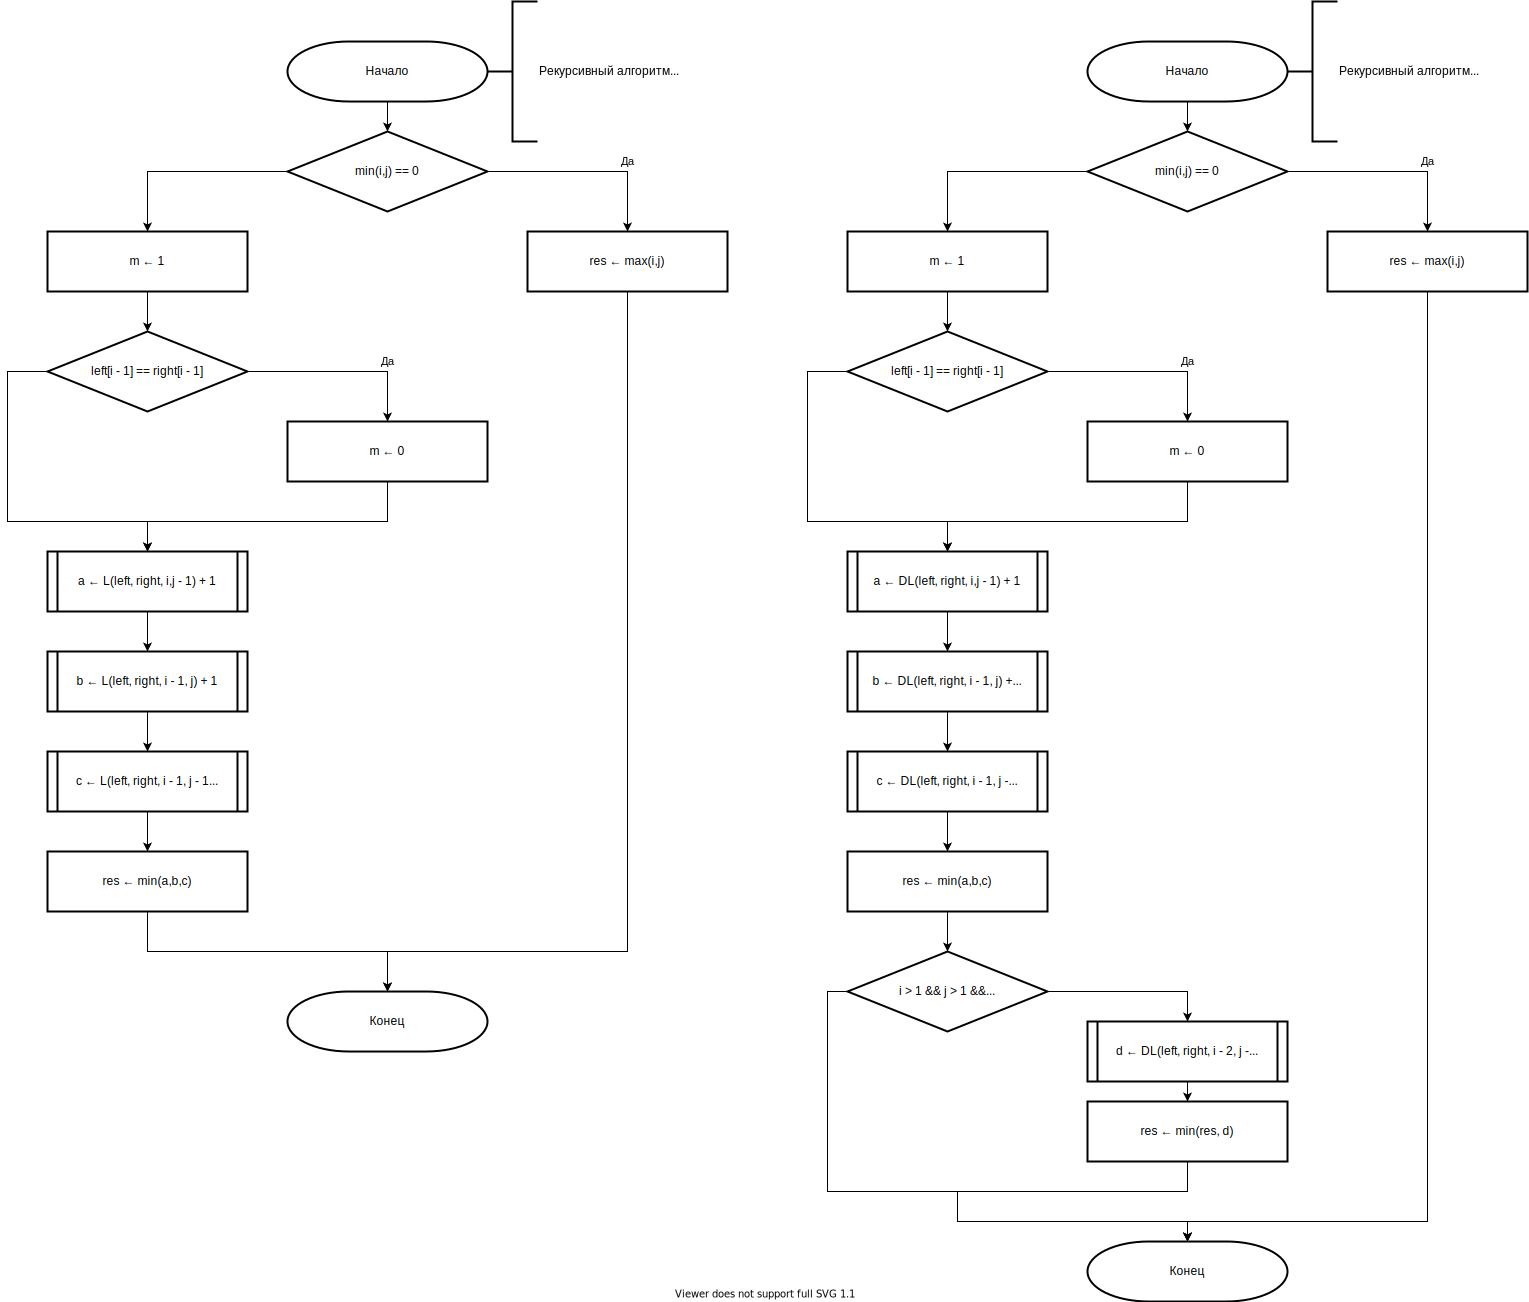
\includegraphics[width=1\columnwidth]{img/flowcharts/1.png}
    \caption{Схема рекурсивных алгоритмов Левенштейна и Дамерау--Левенштейна}
    \label{fig:scheme_algo_recursive}
\end{figure} 

\begin{figure}[h]
    \centering
    \includegraphics[width=1\columnwidth]{img/flowcharts/2.png}
    \caption{Схема рекурсивного алгоритма Левенштейна с кэшированием}
    \label{fig:scheme_algo_cache}
\end{figure} 

\begin{figure}[h]
    \centering
    \includegraphics[width=1\columnwidth]{img/flowcharts/3.png}
    \caption{Схема итеративного алгоритма Левенштейна}
    \label{fig:scheme_algo_iterative}
\end{figure} 


\clearpage
\section{Вывод}
На основе теоретических данных, полученные в аналитическом разделе были построены схемы иследуемых алгоритмов.

%%% Local Variables:
%%% mode: latex
%%% TeX-master: "rpz"
%%% End:
